\documentclass[a4paper,11pt]{article}

\usepackage{clrscode}

\usepackage{geometry}
\geometry{
 a4paper,
 left=30mm,
 top=30mm,
}
\usepackage[utf8]{inputenc}

\usepackage{graphicx}
\usepackage[english]{babel}
\usepackage{color}
\usepackage[dvipsnames]{xcolor}
\usepackage[colorlinks=true,urlcolor=blue,citecolor=black]{hyperref}
\usepackage{url}
%\urlstyle{same}
%\urlstyle{rm}
\urlstyle{sf}
%\urlstyle{tt}
\usepackage[font=footnotesize,labelfont=bf]{caption}
\usepackage[labelfont=it,textfont={it},singlelinecheck=on,justification=centering]{caption}
%full name for appendix
\usepackage[title]{appendix}
\usepackage{float}
\setlength{\parindent}{2em}
\usepackage{parskip}
%for code
\usepackage{listings}
%for math
\usepackage{amsmath}
\usepackage{breqn}
\usepackage{pdfpages}
\linespread{1.1}
\setlength{\emergencystretch}{3em}

\usepackage{ifxetex,ifluatex}
\usepackage{etoolbox}
\usepackage{tikz}

\usepackage{framed}

%water mark
\usepackage{eso-pic}

\newcommand{\watermark}[3]{\AddToShipoutPictureBG{
	\parbox[b][\paperheight]{\paperwidth}{
		\vfill%
		\centering%
	\tikz[remember picture, overlay]%
	  \node [rotate = #1, scale = #2] at (current page.center)%
	      {\textcolor{gray!80!cyan!30}{#3}};
	  \vfill}}}
\usepackage{blindtext}
%water mark end


% conditional for xetex or luatex
\newif\ifxetexorluatex
\ifxetex
  \xetexorluatextrue
\else
  \ifluatex
    \xetexorluatextrue
  \else
    \xetexorluatexfalse
  \fi
\fi
%
\ifxetexorluatex%
  \usepackage{fontspec}
  \usepackage{libertine} % or use \setmainfont to choose any font on your system
  \newfontfamily\quotefont[Ligatures=TeX]{Linux Libertine O} % selects Libertine as the quote font
\else
  \usepackage[utf8]{inputenc}
  \usepackage[T1]{fontenc}
  \usepackage{libertine} % or any other font package
  \newcommand*\quotefont{\fontfamily{LinuxLibertineT-LF}} % selects Libertine as the quote font
\fi

\newcommand*\quotesize{60} % if quote size changes, need a way to make shifts relative
% Make commands for the quotes
\newcommand*{\openquote}
   {\tikz[remember picture,overlay,xshift=-4ex,yshift=-2.5ex]
   \node (OQ) {\quotefont\fontsize{\quotesize}{\quotesize}\selectfont``};\kern0pt}

\newcommand*{\closequote}[1]
  {\tikz[remember picture,overlay,xshift=4ex,yshift={#1}]
   \node (CQ) {\quotefont\fontsize{\quotesize}{\quotesize}\selectfont''};}

% select a colour for the shading
\definecolor{mygray}{gray}{0.95}
\colorlet{shadecolor}{mygray}

\newcommand*\shadedauthorformat{\emph} % define format for the author argument

% Now a command to allow left, right and centre alignment of the author
\newcommand*\authoralign[1]{%
  \if#1l
    \def\authorfill{}\def\quotefill{\hfill}
  \else
    \if#1r
      \def\authorfill{\hfill}\def\quotefill{}
    \else
      \if#1c
        \gdef\authorfill{\hfill}\def\quotefill{\hfill}
      \else\typeout{Invalid option}
      \fi
    \fi
  \fi}
% wrap everything in its own environment which takes one argument (author) and one optional argument
% specifying the alignment [l, r or c]
%
\newenvironment{shadequote}[2][l]%
{\authoralign{#1}
\ifblank{#2}
   {\def\shadequoteauthor{}\def\yshift{-2ex}\def\quotefill{\hfill}}
   {\def\shadequoteauthor{\par\authorfill\shadedauthorformat{#2}}\def\yshift{2ex}}
\begin{snugshade}\begin{quote}\openquote}
{\shadequoteauthor\quotefill\closequote{\yshift}\end{quote}\end{snugshade}}


\usepackage{listings}
\lstdefinestyle{myListStyle}{
  numbers=left,
  stepnumber=1,
  numbersep=10pt,
  tabsize=2,
  showspaces=false,
  showstringspaces=false
}

\usepackage[dvipsnames]{xcolor}
\usepackage{listings}

\newcommand\YAMLcolonstyle{\color{darkgray}\mdseries}
\newcommand\YAMLkeystyle{\color{black}\bfseries}
\newcommand\YAMLvaluestyle{\color{gray}\mdseries}

\makeatletter

% here is a macro expanding to the name of the language
% (handy if you decide to change it further down the road)
\newcommand\language@yaml{yaml}

\expandafter\expandafter\expandafter\lstdefinelanguage
\expandafter{\language@yaml}
{
  keywords={true,false,null,y,n},
  keywordstyle=\color{darkgray}\bfseries,
  basicstyle=\YAMLkeystyle,                                 % assuming a key comes first
  sensitive=false,
  comment=[l]{\#},
  morecomment=[s]{/*}{*/},
  commentstyle=\color{black}\ttfamily,
  stringstyle=\YAMLvaluestyle\ttfamily,
  moredelim=[l][\color{orange}]{\&},
  moredelim=[l][\color{magenta}]{*},
  moredelim=**[il][\YAMLcolonstyle{:}\YAMLvaluestyle]{:},   % switch to value style at :
  morestring=[b]',
  morestring=[b]",
  literate =    {---}{{\ProcessThreeDashes}}3
                {>}{{\textcolor{red}\textgreater}}1
                {|}{{\textcolor{red}\textbar}}1
                {\ -\ }{{\mdseries\ -\ }}3,
}

% switch to key style at EOL
\lst@AddToHook{EveryLine}{\ifx\lst@language\language@yaml\YAMLkeystyle\fi}
\makeatother

\newcommand\ProcessThreeDashes{\llap{\color{cyan}\mdseries-{-}-}}



%opening
\title{\LARGE The Qitmeer White Paper:\\
	\Large The guardian of trust. The core network of the Halalchain}
\author{
	Qitmeer team\\
		\small\href{mailto:paper@qitmeer.io}
			{\nolinkurl{paper@qitmeer.io}}
	}
\date{\today\\\small Version 0.1}
\begin{document}

%% Cover end
\clearpage
\pagestyle{plain}

\maketitle

%\watermark{60}{10}{qitmeer.io}

\begin{abstract}
Bitcoin\cite{bitcoin} was born with revolution, and it opened a new world that currency issuance becomes open and fair by a cryptography-based decentralized payment network. Further on, the underlying ledger mechanism of Bitcoin, i.e. blockchain, was found capable of playing a significant role in the financial field due to its tamper resistance. Islamic finance, as a significant member of world finance, is also experiencing blockchain reshaping.

With the arrival of 10-years birth of bitcoin, the blockchain infrastructure is facing various challenges from technical aspects. Qitmeer regards openness,     fairness, fault tolerance, scalability as the core metrics to assess a promising blockchain paradigm, and a blockchain system achieved a desirable balance among these metrics is regarded as Classical Blockchain Setting.

Qitmeer Consensus picks SPECTRE\cite{SPECTRE} as its fundamental protocol. SPECTRE is a fast\-confirmation and high\-throughput BlockDAG protocol, which guarantees high performance in a payment network. Additionally, Qitmeer introduces another high\-throughput BlockDAG protocol GhostDAG\cite{GhostTDAG}, which is highlighted on unprecedentedly supporting transactions linearly ordering, to circumvent SPECTRE's weak liveness and provide ordering service for the fair scheme of the reward system. Qitmeer Consensus is compliant with Classical Blockchain Setting - it could enter and leave network freely by Proof-of-Work, and the collaboration model of DAG ledger guarantees that miners gain rewards consistent with their devotion, 50\% faulty tolerance as secure as bitcoin, robust scalability that is only subject to physical network limit. The mining algorithm is also a vital source of fairness other than consensus algorithm per se. Cuckoo Ring is a graph theory based proof-of-work mining algorithm and is practically ASIC resistant due to memory-hard calculation.

To be Sharia-Compliant, Qitmeer originates a UTXO-based unique token insurance scheme, which has effectively answered two main concerns: Intrinsic Value and Assets Authentication. Issuing a certain amount of assets must consume a certain amount of the native currency; moreover, entities must be warranted a license to issue assets.

Qitmeer devises a family of specifications and protocols to embrace the whole Isamlic financial ecosystem, such as wallet and miners. As for interoperability, Qitmeer calls for utilizing cross-chain protocols to integrate various cryptocurrencies and offer reliable off-chain smart contract services.


\end{abstract}

\section{Introduction}

\subsection{Background}
Trust is the cornerstone of finance. In traditional approaches, multiple unacquainted parties require a trustworthy third party to guarantee the security of transactions. However, this third party is centralized and subject to single point failure and unlikely to guarantee its honesty.

Bitcoin is an open P2P network, that is to say, no centralized server exists, and each node can join or leave the network freely. The calculation-heavy but validation-easy Proof-of-Work consensus is designed to ensure nodes gain rewards relative to their contribution to the network's running and security, which is supposed to be fair — Bitcoin's disruption to drives tons of researches on its working mechanism. Bitcoin has a hash-list-like ledger to guarantee tamper resistance, further on the concept 'BlockChain' is introduced to represent this mechanism and commonly accepted. Owing to trustlessness and tamper resistance, more and more applications of blockchain occur in the financial field. Blockchain is reshaping finance.

However, with the arrival of 10-years birth of bitcoin, the blockchain infrastructure is facing various challenges from technical aspects and has been deviating its original intention. Bitcoin is no longer decentralized, the top 5 mining pool has controlled majority hash power and would be easy to carry on an attack if they found a reason to. Miners have to join mining pools since the opportunity cost is much higher than their contribution; in other words, Bitcoin is not fair any more. Bitcoin does not scale, seven transactions per second throughput, one hour confirmation time, high cost of the transaction fee, far from promising as a global payment network.

Bitcoin needs reform to return its original intention. Countless solutions arise and claim themselves having solved all these problems. However, few achieved indeed, just trading off one metric with another, e.g. sacrifice decentralization, which is a core source of security, for scalability. So, what the original intention of bitcoin truly is, Qitmeer has its definition and names it as Classical Blockchain Setting, it is also the design philosophy of Quitmeer.

\subsection{Classical Blockchain Setting}
Too many blockchain mutants and each has its definition of blockchain. Quitmeer respects bitcoin's vision, Qitmeer deems it is composed of 4 components and names it as Classical Blockchain Setting.

\subsubsection{Open}
Openness is the critical difference between permissioned and permissionless blockchain, so every node should join and leave the network freely.

\subsubsection*{Predefined special roles}
An open network allows different role, in the bitcoin network, nodes could choose to be an SPV node, full node or miner with freedom, so from the protocol's aspect, bitcoin is open. Whereas, in Delegated Proof-of-Work, the block producers are voted outside of the chain and predefined as configuration, apparently not open enough.

\subsubsection*{Practically close}
Though bitcoin is open according to the protocol, it is close in practical. Miners are no longer independent and have to join mining pools, and this trend is getting worse.


\subsubsection{Fair}
Fairness means that the rewards should be consistent with the contribution; in other words, Incentive-Compatible.

\subsubsection*{Opportunity Cost}
The expectation of rewards between standalone mining and pool mining is equal in terms of probability. The point is, their opportunity cost is considerably high - either mine a block to get a dramatically high reward or wait a long time without any return. So, they have to turn to the mining pool to have a stable incentive.

\subsubsection*{Cost Efficiency}
It is mainly referring to mining cost. Mining cost mainly includes the electricity price and mining efficiency, and the latter is much more critical due to ASIC. ASIC is customized to direct a specific mining algorithm, so the mining efficiency per unit of cost is much higher than generalized computers. For instance, the hash rate per dollar for AntMiner S9 is about 20000 times greater than for GTX570; it is nearly impossible for a personal computer to win the hash rate competition.

\subsubsection{Secure}
The security is how robust the network is to sustain the attack, mainly referring to overrun a confirmed transaction.

\subsubsection*{Decentralization}
Decentralization is the most significant difference for bitcoin to be compared with traditional payment network. Decentralization could avoid single point failure; also, it is almost impossible to collude with the majority of all nodes in a fully decentralized network.
\subsubsection*{Fault Tolerance}
The network should be resilient to a certain proportion of misfunctioning resources, and  Tolerance is the upper bound of the percentage. In a decentralized network, 50\% fault tolerance is the ideal case according to the majority law.

\subsubsection{Scalable}
A network that can offer relatively stable services with its scale increasing is considered scalable. Blockchain network includes the following services:
\subsubsection*{Throughput}
How many transactions per second when network is scaling. Bitcoin's throughput is upper bound to 7 TPS, no matter how many nodes are there in the network.
\subsubsection*{Confirmation}
How long does the recipient to wait until his transaction is believed unlikely to be overrun? The waiting time should not increase with networking scaling.
\subsubsection*{Cost}
The main component of cost is transaction fee, and it should be reasonable, it would make payment impractical if too high, whereas be subject to sybli attack if too low. With the mining difficulty increasing, Bitcoin transacation fee is getting higher and higher, and it won't be suitable to serve as a global payment network as it aimed to, up to the time this paper finished, the average price of bitcoin is rough 2\$ . [https://bitcoinfees.info/]

\subsection{Specification}
Qitmeer's specification is designed to abide by Classical Blockchain Setting
\subsubsection{Openess}
Qitmeer is an open network; it uses proof-of-work to join the network freely and use BlockDAG protocol to avoid the risk of mining pools centralization.
\subsubsection*{Proof of Work}
Proof-of-Work is the openest way so far to join a blockchain network because the only resource required to contribute to is electricity, which every node has owned. Besides, this resource is physical; in other words, it is non-duplicatable.
\subsubsection*{No Predefined Nodes}
 Quitmeer doesn't have predefined sepcial nodes , i.e. super nodes.
\subsubsection{Fairness}
BlockDAG is fair because it is a collaboration model other the competition model of blockchain.
\subsubsection*{Mining Pool Resistance}
Mining pools centralization is the consequence of high opportunity cost, which is the consequence of the competition model. Qitmeer's BlockDAG-based protocol SPECTRE is a collaboration model, the opportunity cost of standalone mining is equal to that of pool mining, so it will not be necessary to join a mining pool, which would lead to the risk of centralization.
\subsubsection*{Anti-ASIC Mining Algorithm}
Cuckoo Cycle is a graph-theoretic proof-of-work algorithm and prevails for ASIC resistance. Qitmeer employs this algorithm to guarantee that no one has too much mining efficiency advantage.
\subsubsection{Security}
Security is the first code in Quitmeer, and it is a fully decentralized and 50\% fault tolerant, which is the most stringent criteria; thus, there is no security sacrifice for other metrics.
\subsubsection*{Fully Decentralization}
All the nodes in the Qitmeer's network are peer nodes and can participate in consensus.
\subsubsection*{50\% Faulty Tolerance}
The malicious adversary has to posses 50\% hash power to control the network. Either in SPECTRE or GhostDAG, the fault tolerance is irrelevant with the throughput, whereas the security is inversely propagational to throughput in bitcoin.

\subsubsection{Scalability}

Qitmeer's hybrid BlockDAG protocols scales, fast confirmation, high throughput, low transaction fee, all these features ensure Qitmeer will be running stably in a considerable long time.
\subsubsection*{Fast Confirmation}
SPECTRE is a speedy confirmation BlcokDAG protocol, and Qitmeer uses as its consensus algorithm.
\subsubsection*{High Throughput}
SPECTRE is a BlcokDAG protocol, and the throughput could grow up to the network's physical metrics, such as network bandwidth or propagation delay.
\subsubsection*{Low Cost}
Strictly speaking, the cost is not scaling since the transaction fee is increasing slightly with the network growing. However, the average cost will keep relatively low and acceptable for a long time. So, from the reasonableness aspect, the cost scales.

\section{Qitmeer Token Design}
The existing blockchains are not able to be essentially Sharia-Compliant because they don't take it into consideration when they initiate their design. Qitmeer takes Sharia-Compliance into account as the very beginning and has redesigned an effective solution, namely OP\_TOKEN.

\subsection{Overview}
\subsubsection{Problem definition}

Blockchains are ought to respect two main concerns to comply Sharia:

\subsubsection*{Intrinsic Value}
Assets must have underlying value and cannot be created out of thin air. On existing token issuance platforms like Ethereum\cite{Ethereum}, individuals can issue a token of arbitrary amount without any foundation.

\subsubsection*{Assets Authentication}
Should not allow issuarance of illegitimate assets. Existing blockchains are too unrestricted to have necessary assets authentication.
\subsubsection{Related works}

The $\texttt{OP\_TOKEN}$ is inspired by Color coin idea, which represents and manages real-world assets on top of the Bitcoin by using $\texttt{OP\_RETURN}$, and the OP\_GROUP, a referenced implementation of issuing assets designed by Andrew Stone.

The OP\_TOKEN fit various practical scenarios with unique features like asset compliable and value relevent. There are some related concepts in the details below:

\subsubsection{UTXO}

UTXO represents Unspent Transaction Output. In other words, there are no accounts in Qitmeer. What users have and spend are a bunch of unspent transaction outputs, and we could come up with the balance by summing up them.

\begin{figure}[hbt]
	\centerline{%
	   \resizebox{0.8\textwidth}{!}{\includegraphics{figures/UTXO}}%
	}
\caption{utxo model}
\end{figure}

The first transaction tx1 has three outputs with the first spent, so  tx1 has 2+3=5 coins balance.

The second transaction, tx2 spends the 2 UTXOs of tx1 and pays to 3 addresses and creates three new UTXOs.

Note: now the old UTXOs (of tx1) are no longer UTXO so cannot be spent later.

\subsubsection{Script system}

The mechanism behind how users spend their UTXOs is to execute a particular script. The output stores half of the script and we have to present the other half and combine both to verify if we could spend the money. The former half is called locking script, like a locked treasure box, and the latter is unlocking script, like the only key to the box.

Let us take a look at the typical instance of  Pay-2-Public-Key-Hash(P2PKH)\cite{P2PKH}

Locking Script in UTXO:

\begin{lstlisting}
OP_DUP OP_HASH160 <PUBLIC_KEY> OP_EQUALVERIFY OP_CHECKSIG
\end{lstlisting}

Unlocking Script in a newly created transaction:

<Signature><PublicKey>

Combine unlocking script with locking script:

<Signature><PublicKey> OP\_DUP OP\_HASH160 <PUBLIC\_KEY> OP\_EQUALVERIFY OP\_CHECKSIG

This whole script consists two steps
1. <PublicKey>  OP\_HASH160 <PUBLIC\_KEY> OP\_EQUALVERIFY
	To verify if the public key in the unlocking script matches that in the locking script.
2.  <Signature><PublicKey> OP\_CHECKSIG
	To check if the signature is valid.


\subsubsection{Colored coins and Tether}

Colored Coins\cite{ColoredCoins} is a method to represent assets on top of the blockchain so that it can leverage the tamper-proof capability of blockchain. It uses tx-script operation $\texttt{OP\_RETURN}$ to interrupt script execution early, so we can add information on the assets after it without violating the script validation.

Locking Script:
\begin{lstlisting}
OP_RETURN <DATA>
\end{lstlisting}

The stable coin Tether\cite{Tether} (USDT) also uses OP\_RETURN based OMNI Layer protocol to define the asset on the bitcoin.

Here are a typical USDT transaction and details of its protocol design


\lstset{basicstyle=\tiny,style=myListStyle}
\begin{lstlisting}
OP_RETURN 6f6d6e69000000000000001f00000015c9054900
\end{lstlisting}


\begin{figure}[hbt]
	\centerline{%
	   \resizebox{0.8\textwidth}{!}{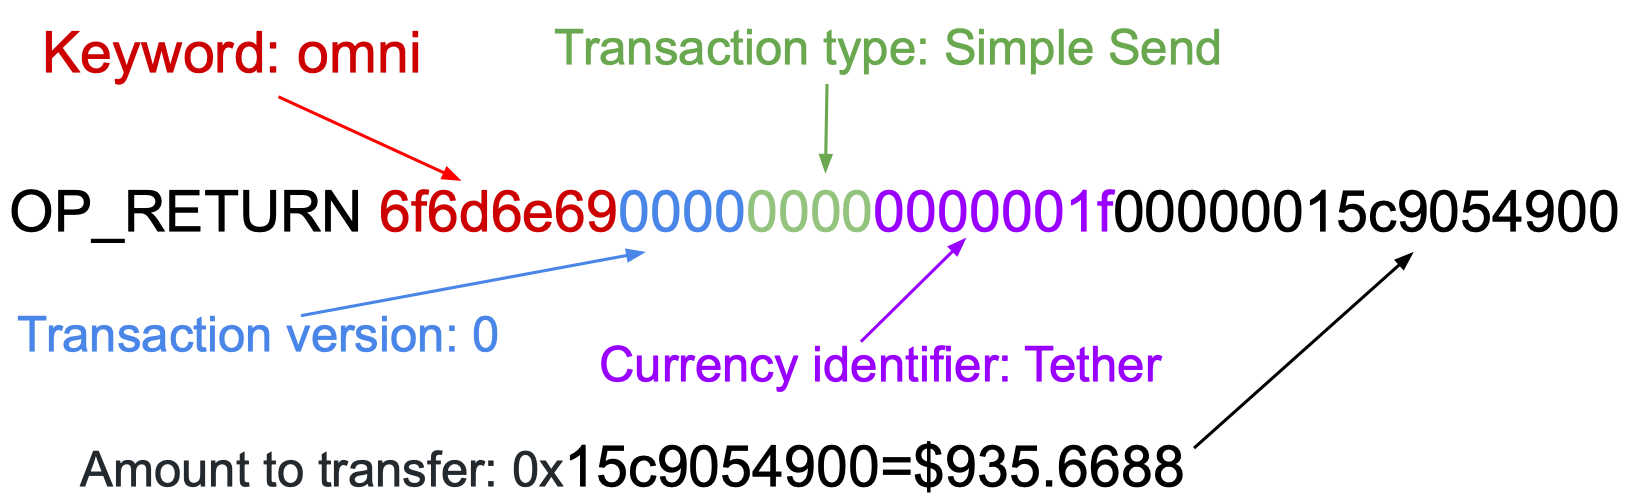
\includegraphics{figures/USDT}}%
	}
\caption{USDT}
\end{figure}


%[ref][https://www.blockchain.com/btc/tx/efc50d9e1f23e687e304cfca4ef2c5412b67d5737888ff80a0cbb6853cd865c]



\subsubsection{OP\_GROUP}
The OP\_RETURN scheme is more suitable to apply on mature blockchain since it does not change the underlying blockchain protocol and will not risk forking. However, the weakness is that miners cannot verify its protocol, so there would be some security risks.

OP\_GROUP\cite{OP_GROUP} is a proposal of assets issuance on Bitcoin Cash (BCH)\cite{BCH} from Bitcoin Unlimited (BU). OP\_GROUP supports token issuance, transfer, destroy, and so on forth. Since OP\_GROUP is an extension to the BCH script system,  it is part of the BCH protocol. Thus miners can do the verification, which is more reliable.

The basic “colored” pay 2 public key hash script would be like:

\lstset{basicstyle=\tiny,style=myListStyle}
\begin{lstlisting}[numbers=none]
OP_DATA(group address)
OP_GROUP
OP_DROP
OP_DUP
OP_HASH160
OP_DATA(pubkeyhash)
OP_EQUALVERIFY
OP_CHECKSIG
\end{lstlisting}

The main difference is simple, just adding a group address to distinguish different groups, and other operations, such as create and destroy assets, are similar.

% [ref]https://medium.com/@g.andrew.stone/bitcoin-scripting-applications-representative-tokens-ece42de81285

\subsection{OP\_TOKEN Design}

\subsubsection{Overview}

There is a unique token named LICENSE in OP\_TOKEN. With public credibility, Renowned experts or organizations hold licenses. Any entity planning to issue a token needs to be warranted a license.  Peers can transfer licenses as they are also tokens. The transfer history is public and immutable, so the originator must be very cautious in case of transferring to a wrong hand.

\subsubsection{Issuance of License}

Licenses are all generated in the genesis block and distributed to C preserved committee members. One smallest unit (SAND) can represent a license, one block has M coins, one coin= N SAND, so we have M*N license in total, which is sufficient for asset issuance.


\begin{lstlisting}[language=yaml, numbers=none,basicstyle=\footnotesize]
# C = 100, M = 10, N = 10^8 (M*N = 10 billion),
# all examples are based on this setting
# Ex1: Distribute licenses to the commitee,
# M*N/C = 100 million for each member.
---
INPUTS:
	INPUT:
		PREVIOUS_OUTPUT: # (COINBASE of GENESIS)
			S: "DUP HASH160 [GEN] EQUALVERIFY CHECKSIG"
			V: 10000000000
		S: "[SIG] [GEN_PK]"
OUTPUTS:
	OUTPUT:
		S: "[LIC] TOKEN DROP DUP HASH160 [COMM1] EQUALVERIFY CHECKSIG"
		V: 100000000
	# ... ... (COMMITTEE MEMBER 2~99)
	OUTPUT:
		S: "[LIC] TOKEN DROP DUP HASH160 [COMM100] EQUALVERIFY CHECKSIG"
		V:100000000
	OUTPUT:
		S: "RETURN [DATA]"
		V: 0
\end{lstlisting}



\subsubsection{Warrant a license}

Organizations must be warranted a license to issue assets. They can request a license from any committee member (C.M.). Once the license is granted and approved, they will receive a particular token transfer from the C.M. and the token is the license.

\lstset{basicstyle=\tiny,style=myListStyle}
\begin{lstlisting}[language=yaml, numbers=none,basicstyle=\footnotesize]
# Ex2: C.M. warrant a license to the issuer (ISS),
# note the license change will go back to the C.M.
---
INPUTS:
	- INPUT:
			PREVIOUS_OUTPUT:
				S: "[LIC] TOKEN DROP DUP HASH160 [COMM] EQUALVERIFY CHECKSIG"
				V: 100000000
			S: "[SIG] [COMM_PK]"
OUTPUTS:
	- OUTPUT:
			S: "[LIC] TOKEN DROP DUP HASH160 [ISS] EQUALVERIFY CHECKSIG"
			V: 1
	- OUTPUT: # License change
			S: "[LIC] TOKEN DROP DUP HASH160 [COMM] EQUALVERIFY CHECKSIG"
			V: 99999999
	- OUTPUT:
			S: "RETURN [DATA]"
			V: 0
\end{lstlisting}

\subsubsection{Issuance of assets}
Once warranted a license, organizations can issue assets; however, they cannot set the token amount arbitrarily. Instead, to issue a certain amount of assets requires converting the same amount of  SANDs. Qitmeer calls this process as  "token mint". Just like the case in reality,  to mint a gold coin requires the same weight of gold sands, tokens need the same amount of SANDs.

The first benefit of this issuance system is to guarantee tokens' elementary intrinsic value; thus, it would significantly mitigate the price fluctuation. Another advantage is that tokens and native currency are no longer isolated islands of value; they are running is the same ecosystem, which would improve the liquidity and make the whole network healthier.

\lstset{basicstyle=\tiny,style=myListStyle}
\begin{lstlisting}[language=yaml, numbers=none,basicstyle=\footnotesize]
# Ex3: Convert 100000000 native SANDs, i.e. 1 Coin,
# to 100000000 sands of the new token,
# note the license will go back to the issuer for future issurance.
INPUTS:
	- INPUT:
			PREVIOUS_OUTPUT: #(1 LICENSE)
				S: "[LIC] TOKEN DROP DUP HASH160 [ISS] EQUALVERIFY CHECKSIG"
				V: 1
			S: "[SIG] [LIC_PK]"
	- INPUT:
			PREVIOUS_OUTPUT: #(1 Qitmeer Coin)
				S "DUP HASH160 [COIN] EQUALVERIFY CHECKSIG"
				V: 100000000
			S: "[SIG] [COIN_PK]"
OUTPUTS:
	- OUTPUT: # License returns to the issuer
			S: "[LIC] TOKEN DROP DUP HASH160 [ISS] EQUALVERIFY CHECKSIG"
			V: 1
	- OUTPUT:
			S: "[TOK] TOKEN DROP DUP HASH160 [PK] EQUALVERIFY CHECKSIG"
			V: 100000000
	- OUTPUT:
			S: "RETURN [DATA]"
			V: 0
\end{lstlisting}

\subsubsection{Transfer of the Assets}

Parties can transfer assets to each other. Moreover, we could transfer multiple assets within one transaction. The transaction needs to ensure the input sum of each asset equals the output sum of each asset.

\lstset{basicstyle=\tiny,style=myListStyle}
\begin{lstlisting}[language=yaml, numbers=none,basicstyle=\footnotesize]
# Ex4: Alice exchanges her 100 RMB token with Bob's 20 USD token.
INPUTS:
	- INPUT:
			PREVIOUS_OUTPUT:
				S: "[RMB] TOKEN DROP DUP HASH160 [A_PKH] EQUALVERIFY CHECKSIG"
				V: 100
			S: "[A_SIG] 0X83 [A_PK]"
	- INPUT:
			PREVIOUS_OUTPUT:
				S: "[USD] TOKEN DROP DUP HASH160 [B_PKH] EQUALVERIFY CHECKSIG"
				V: 20
			S: "[B_SIG] 0X83 [B_PK]"
OUTPUTS:
	- OUTPUT:
			S: "[USD] TOKEN DROP DUP HASH160 [A_PKH] CHECKSIG"
			V: 20
	- OUTPUT:
			S: "[RMB] TOKEN DROP DUP HASH160 [B_PKH] CHECKIG"
			V: 100
\end{lstlisting}


\subsubsection{Melt Token}

Melt is the reversed process of mint, i.e., conversion from tokens to native currency. The total amount of sands is constant, either in the form of Native Sand or Token Sand. So it is forbidden to destroy a token and only allowed to convert tokens. Issuers can melt their coins to reduce the liquidity in order to keep the price stable, which is practical to implement stable coins.


Melt guarantees the tokens fundamental value, just like the minimum value of a gold coin is the same weight of gold.

\lstset{basicstyle=\tiny,style=myListStyle}
\begin{lstlisting}[language=yaml, numbers=none,basicstyle=\footnotesize]
# Ex5: Melt 100 token sands into 100 native sands
INPUTS:
	- INPUT:
			PREVIOUS_OUTPUT:
				S: "[TOK] TOKEN DROP DUP HASH160 [ISS] EQUALVERIFY CHECKSIG"
				V: 100
			S: "[SIG] [ISS_PK]"
OUTPUTS:
	- OUTPUT:
			S: "DUP HASH160 [COIN] EQUALVERIFY CHECKSIG"
			V: 100
	- OUTPUT:
			S: "RETURN [DATA]"
		V: 0
\end{lstlisting}


\section{Consensus Protocol}


\subsection{From BlockChain To BlockDAG}
BlockChain represented by Bitcoin does not scale due to protocol restrain. On Nakamoto Consensus, i.e., longest-chain rule, 1 MB block size and 10 minutes block rate confine bitcoin to reach only 7 TPS  theoretical throughput regardless of the bandwidth and propagation delay.

The most intuitive way to increase scalability is to shorten block time or enlarge block size. The reason why Satoshi did not adopt is that it brings forks, and they distract the hash power from the main chain, thus causing security vulnerability.

GHOST protocol introduces heaviest-tree consensus to keep forks without sacrificing security. Note that here BlockChain has transformed into a BlockTree. Since the largest subtree has concentrated the majority hash power, the security is as high as bitcoin. The main chain is the path,  i.e. a blockchain from the genesis to leaf, with the highest number of descendants, other blocks are off-chain blocks. Only main chain blocks contribute throughput, off-chain blocks help strengthen the security.

BlockTree has dramatically increased the throughput because of the higher Block Rate or Size. However, there is still a waste of the transactions of off-chain blocks, which should contribute to the throughput as well. Inclusive protocol proposes a new data structure of ledger, where every block confirms every unconfirmed block. This improvement upgrades a BlockTree to a BlockDAG.

Through the history from BlockChain to BlockDAG, we may infer that BlockChain is just the particular case on low throughput of BlockDAG, they are, in essence, the same. So, it is the scaling approach whose paradigm is closest to bitcoin. The apparent benefit is that it would be robust since it can inherit all the long-time-proved stable features of bitcoin. Besides, this approach is scalable infinitely in terms of protocol, only limited by physical limits, like bandwidth. A robust public chain itself is the optimal basis for incorporating further scaling solutions, such as sharding and state-channels, so BlockDAG is the preferred scaling solution of Qitmeer.


\begin{figure}[hbt]
	\centerline{%
	   \resizebox{0.8\textwidth}{!}{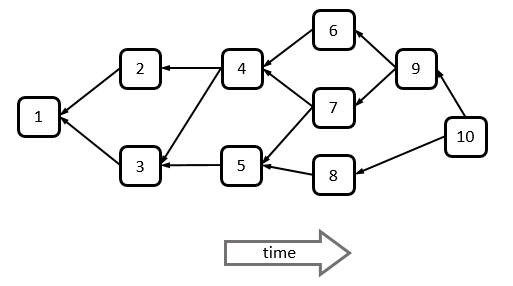
\includegraphics{figures/DAG.png}}%
	}
\caption{DAG}
\end{figure}

\subsection{Consensus}

Qitmeer adopts a hybrid consensus that combines SPECTRE and GHOSTDAG  in order to achieve fast confirmation and high throughput.

\subsubsection{SPECTRE}
SPECTRE\cite{SPECTRE} is a block-DAG based protocol that achieves fast confirmation and high
throughput with 50\% attack resilience. SPECTRE guarantees safety, which means a
transaction is unlikely to be reversed once it is accepted. Also, SPECTRE guarantees fast confirmations for honest users rather than all users; in other words, weak liveness.

There is a trade-off between liveness and fast confirmation; SPECTRE prioritizes
the latter since weak liveness only affects malicious users. SPECTRE is appropriate for payment model. Only malicious users launch double spends, so only their
transactions are likely to be delayed indefinitely.

SPECTRE is a stateless transaction model, so there is no need to gain a
total ordering over all the blocks. Only when two blocks conflicting
that a pairwise ordering is needed.

SPECTRE employs a voting algorithm to decide which block wins when two blocks
conflict. Suppose block $x$ has a conflicting transaction with another
transaction in block $y$, and also suppose that block $z$ is voting on them with
the following rules:

\begin{enumerate}
	\item If $z$ is in $x$'s future but not in $y$'s future, $z$ votes for
		$x$ in favor of $y$, denoted as $x \prec y$, and vice versa.
	\item If both $x$ and $y$ are in the past of $z$, then $z$ follows the majority votes in its past.
	\item If neither $x$ nor $y$ is in the past of $z$, then $z$ follows the majority votes in its future.
	\item Both $x$ and $y$ vote for themselves unless one is in the past of
		the other.
\end{enumerate}


Here's an example of how a new block (number 12 in the figure below) votes:

\begin{figure}[ht]
	\centerline{%
	   \resizebox{0.8\textwidth}{!}{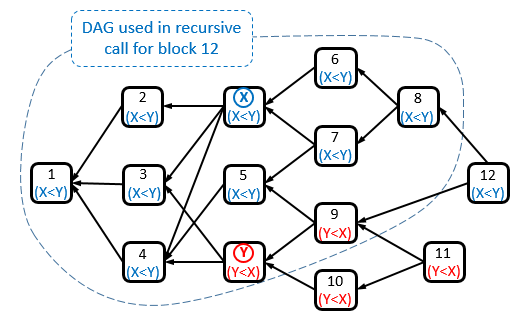
\includegraphics{figures/SPECTRE}}%
	}
\caption{An example of the voting procedure in the DAG for blocks $x$ and $y$ in SPECTRE}
\end{figure}

According to rule 4, block $x$ votes for $x \prec y$, block $y$ votes for $y
\prec x$.

According to rule 1, blocks 6, 7 and 8 vote for $x \prec y$, blocks 9, 10 and 11
vote for $y \prec x$.

According to rule 2, block 12 votes according to its past. Since not all blocks
of its past have voted, we change global view to block 12's local view, which
means block 10 and 11 are excluded.

According to rule 3, block 5 votes for $x \prec y$, since the majority of its
future vote in favor of $x$ over $y$ (blocks 7, 8 versus block 9). Note that the
current view is block 12's local view and block 11 is exculded, so we cannot
take its vote.

Also according to rule 3, blocks 1\textasciitilde4 vote for $x \prec y$.

Now all the blocks in block 12's past have voted. Block $x$ gets 10 votes. Block
$y$ gets 2 votes. Block 12 follows the majority and votes for $x \prec y$ thus.


\subsubsection*{Confirmation Time}

The SPECTRE paper provides two ways of accepting (confirming) a block, i.e. the
offline way and the online way. The online way is more straightforward. The
simulation results of the paper also adopted the online way. Qitmeer adopts the same
way.

When a node $v$ receives a block $x$, it loops to calculate the online risk of
the block. It accepts the block when the risk is smaller than a given threshold
$\epsilon$. The online confirmation time of block $x$ in node $v$ is the time
since $x$ is received by $v$ until $x$ is accpeted by $v$.

The following algorithm below calculates the online risk of block $x$ in
$G_t^v$, where $G_t^v$ is the block DAG that $v$ observes at time $t$.

\begin{codebox}
\Procname{\proc{Risk}$(G_t^v, x)$}
\li \If $time\_now < publication(x)$
\li   \Then
        \Return 1
      \End
\li $T \gets time\_now - received^v(x)$
\li $G_x \gets G_{received^v(x) + 2 \cdot d} \cup future(x, G_t^v)$
\li $g \gets \min_{x' \in \overline{ainticone}(x,G_x)} |future(x',G_x)|$
\li \Return $risk\_hidden(T,g)$
\end{codebox}

The formula $risk\_hidden(T,g)$ is defined as:

$$
risk\_hidden(T,g) := \sum_{l=0}^{\infty} \pi(l) \sum_{m=0}^{\infty} Poiss((T + 2
\cdot d) \cdot \alpha \cdot \lambda, m) \cdot \left(\frac{\alpha}{1 -
\alpha}\right)^{(g - l - m)^+},
$$

where

\begin{itemize}
	\item $d$ is the upper bound on the recent delay diameter in the network,
	\item $\alpha$ is the attacker’s relative computational power,
	\item $\lambda$ is the block creation rate,
	\item $Poiss(a, b)$ is defined as $e^{-a} \cdot \frac{a^b}{b!}$,
	\item $x^+$ is defined as $\max\{0, x\}$,
	\item and $\pi$ is the stationary distribution which we will explain below.
\end{itemize}

$risk\_hidden(T,g)$ upper bounds the probability that block $x$ is preceded by
some attacker’s block $y$ in pairwise order, where $y$ is published later than
$x$.

$\pi$ is actually a vector. Informally, it is the statistical distribution of
how much more blocks attacker nodes have created than honest nodes have created
since block $x$ is published, which is called gap in the SPECTRE paper. $\pi(l)$
is the probability that the value of gap is $l$.

The value of gap changes as time goes on, forming a random walk which induces an
ergodic Markov chain. Theorietically, it could be any integer ranging from
negative infinity to positive infinity. In the worst case, it is always
non-negative. Only when the gap is non-negative is there a risk for block $x$ to
be received less or equal votes than some attacker’s block $y$ which is
published later than $x$, so that $y$ precedes $x$ in pairwise order. This is
why in the formula of $risk\_hidden$ the index $l$, i.e. the value of gap,
starts out equal to 0 instead of negative infinity.

Since the random walk of $l$ induces an ergodic Markov chain, $l$ has a unique
stationary distribution, which is $\pi$. In order to calculate $\pi$, we need to
calculate the transition probability matrix of the random walk.

Suppose that the value of $l$ ranges from 0 to $N$, where $N$ is infinity in the
above definition. We define the transition probability matrix as an $N$ by $N$
matrix $T$. We also denote by $\delta := \alpha \cdot \lambda \cdot d$. For all
$1 \leq l < N - 1$, $T_{l-1,l} = 1 - \alpha, T_{l+1,l} = \alpha$, and for $l = N
- 1$: $T_{l-1,l} = 1 - \alpha, T_{l,l} = \alpha$. The first column of the matrix
is defined by: $T_{0,0} := (1 - \alpha) \cdot e^{-\delta}, T_{1,0} = e^{-\delta}
\cdot \alpha + e^{-\delta} \cdot \delta$, for $1 < l < N - 1$: $T_{l,0} =
e^{-\delta} \cdot \frac{\delta^l}{l!}$, and $T_{N-1,0} = 1 - e^{-\delta} \cdot
\left[\frac{\delta^0}{0!} + \frac{\delta^1}{1!} + \cdots +
\frac{\delta^{N-2}}{(N-2)!}\right]$.  $\pi$ is the eigenvector of $T$
corresponding to the eigenvalue 1, where $\pi(l) \geq 0$ and the sum of $\pi$ is
1.

In practice, $\pi(l)$ is very close to zero when $l$ is very large, so we can
just pick some $N \gg 1$ instead of infinity. Therefore, the formula of
$risk\_hidden$ becomes

$$
risk\_hidden(T,g) = \sum_{l=0}^{N} \pi(l) \sum_{m=0}^{\infty} Poiss((T + 2 \cdot
d) \cdot \alpha \cdot \lambda, m) \cdot \left(\frac{\alpha}{1-\alpha}\right)^{(g
- l - m)^+}.
$$

It is recommended to calculate $\pi$ with some well-tested Markov chain library such
as the markovchain package in R.

The sum of series with index $m$ seems to be a sum of infinite series. However,
for $m > g - l$ we have $(g - l - m)^+ = 0$ and
$\left(\frac{\alpha}{1-\alpha}\right)^{(g - l - m)^+} = 1$.

Therefore, the formula of $risk\_hidden$ can be further converted as below,
where $Poiss_{cdf}$ is the cumulative distribution function (CDF) of Poisson
distribution.

\begin{align*}
risk\_hidden(T,g)
=& \sum_{l=0}^{N}\pi(l)\sum_{m=0}^{\infty}Poiss((T+2 \cdot d) \cdot \alpha \cdot \lambda, m) \cdot (\frac{\alpha}{1-\alpha})^{(g-l-m)^+} \\
=& \sum_{l=0}^{N}\pi(l) (\sum_{m=0}^{g-l}Poiss((T+2 \cdot d) \cdot \alpha
	\cdot \lambda, m) \cdot (\frac{\alpha}{1-\alpha})^{(g-l-m)} + \\
& \sum_{m=(g-l+1)^+}^{\infty}Poiss((T+2 \cdot d) \cdot \alpha \cdot \lambda, m)) \\
=& \sum_{l=0}^{N}\pi(l) ( \sum_{m=0}^{g-l}Poiss((T+2 \cdot d) \cdot
	\alpha \cdot \lambda, m) \cdot (\frac{\alpha}{1-\alpha})^{(g-l-m)} + \\
& (1 - Poiss_{cdf} ((T+2 \cdot d) \cdot \alpha \cdot \lambda, (g-l)^+))).
\end{align*}

With the converted formula we are able to calculate $risk\_hidden$ in numerical way.


\subsubsection{GHOSTDAG}


Since Qitmeer works for payment, in most cases it is
sufficient to provide only partial ordering or pairwise ordering for blocks in
the ledger. However, sometimes we may still need to obtain a total (linear)
ordering of all the blocks, especially when we want to reward blocks based on
their ordering.

Obtaining total ordering for a DAG ledger is not so intuitive as it is for
blockchains since a DAG ledger contains forks, which are caused by various reasons, such as, network
propagation delay, concurrent block creations, faulty miners.
Therefore, as a supplement to the consensus protocol of Qitmeer, we use GHOSTDAG to
obtain the total ordering to reward blocks which appears earlier in the
ordering.

In addition to total ordering, GHOSTDAG also provides Strong Liveness guarantee
to make the consensus protocol more robust, which means both honest blocks and
malicious blocks can be confirmed within a definite time, though it may take a
long time to confirm malicious blocks.

Suppose that the maximal limits of network propagation delay and block creation
rate are constant. It is intuitive that if nodes behave honestly, they form
a subgraph where each block has at most a constant number of forks. We denote
this constant number as $k$. $k$ can be calculated from propagation time and
block creation rate. The subgraph is denoted as a $k$-cluter. The biggest
$k$-cluster is called a blue set. Those blocks outside the blue set are called
red set.

If we can traverse from block $x$ to block $y$ by following the parent
references within each block, then we say that there's a partial order between
$x$ and $y$, and $y$ is prior to $x$. For example in the following figure, we
can traverse from block J to A through B, so there's a partial order between A
and J, and A is prior to J. Note not all blocks have partial orders with other
blocks. For example, there're no partial orders between B, C and D. We call the
block set where no partial order exists an anticone. The size of any anticone in
a $k$-cluster is at most $k$.

\begin{figure}[ht]
	\centerline{%
	   \resizebox{0.8\textwidth}{!}{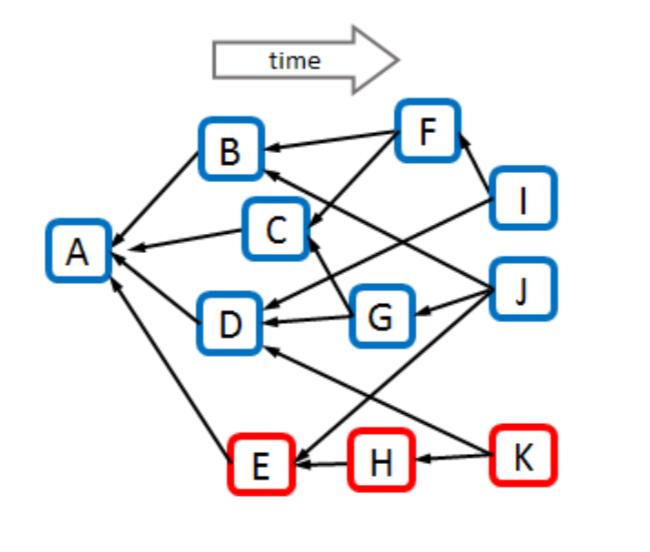
\includegraphics{figures/GHOSTDAG}}%
	}
\caption{GHOSTDAG}
\end{figure}


GHOSTDAG orders the DAG ledger in a way that favours blue blocks and penalizes
red ones. We determine the order between blue blocks according to their partial
orders and some topological sort. Then, for any blue block $B$, add to the order
just before $B$ all of the red blocks in $past(B)$ that weren’t added to the
order yet; these red blocks too should be added topologically. Notice
that for any blue block $B$, the order on blocks in $past(B)$ should remain the
same if we remove from the DAG blocks in $future(B)$.

An example of the output order of the GHOSTDAG procedure on the small DAG ledger
from the figure above is: $(A,D,C,G,B,F,I,E,J,H,K)$. Unfortunately, finding the
maximum $k$-cluster is NP-hard, so GHOSTDAG is therefore of less practical use
for an ever-growing DAG ledger and may cause long confirmation times.
Therefore, we use GHOSTDAG only to implement the reward mechanism of Qitmeer, since
it should be acceptable for a miner to wait for a while to get his or her mining
reward. The confirmation time for a transaction to be accepted is still defined
in the SPECTRE way.

\subsection{Mining Algorithm}
\subsubsection{BlockDAG and Mining}
BlockDAG's collaboration model provides much more fairness than the competition model of BlockChain on the protocol aspect. Every node gets rewards according to its contribution, regardless of how much hash power they possess. Qitmeer considers the fairness benefit even more important than the scalability increase because it represents the spirit of BlockChain. The intention of Nakamoto Consensus is fair - every node votes with electricity; however, only a small bunch of the mining pools have the odds to participate in consensus. Standalone miners suffer huge opportunity cost since they have to wait uncertain time, quite long in most cases, to mine a block to cover their cost; thus finally they have to turn to the mining pools. BlockDAG incorporates every miner's block, so the miners have a strong expectation of their return and then don't have too much willing to join a mining pool.

Apart from the protocol, the mining algorithm is another factor of fairness, so the protocol fairness is of no use without mining fairness. Mining fairness refers to a certain amount of mining cost, i.e. electricity in POW, should derive the relatively equivalent amount of hash power. Practically, the ASIC mining rigs have much more mining efficiency than their prices.

\subsubsection{Cuckoo-Cycle-PoW}
Proof-of-Work(PoW) is used to confirm transactions and produces new blocks, therefore it is a very important engine in PoW cryptocurrencies. PoW must not enable a participant to have a significant advantage over another participant. That is why Satoshi said: "Proof-of-work is essentially one-CPU-one-vote."

However, most widely used proof-of-work algorithms, such as SHA-256, Blake2b, Scrypt, are more efficient on ASIC devices when compared to CPUs and GPUs. This can lead to ASIC owners posses a much larger voting power than CPU and GPU owners. It violates the “one-CPU-one-vote” principle.

We introduce Cuckoo-Cycle-PoW ,a graph-theoretic proof-of-work algorithm. It is ASIC resistant.

Cuckoo-Cycle-PoW is designed to find certain subgraphs in large pseudo-random graphs. This algorithm that we hope turns out to be ASIC resistant. It utilizes almost all parts of commodity hardware (GPUs).

The Cuckoo Cycle POW is the work of John Tromp, it is designed to find certain subgraphs in large pseudo-random graphs. In particular, Search for cycles of specified length L in a bipartite graph with M edges of N nodes. If a cycle is found and the hash difficulty is less than the target difficulty, the cuckoo cycle PoW is completed.


\textbf{Overall flow}

\begin{enumerate}

\item Outer loop

\begin{enumerate}
	\item Build block Header with following values:

		\begin{itemize}
		\item Difficulty: Difficulty target for tx
		\item TxRoot: The merkle root of the tx tree
		\item Timestamp: A Unix time timestamp
		\item Nonce: A 64-bit (8-byte) field whose value is adjusted by miners
		\item ParentRoot: The merkle root of the previous parent blocks (the dag layer)
		\end{itemize}

	\item Set amount of the attempt time, currently configured at 60 seconds, for inner loop.
	\item Set the deadline is equal to the attempt time add the current unix timestamp.
	\item Inner loop

		\begin{enumerate}
			\item Check the header’s hash is the latest header’s hash and the current timestamp less than the deadline.
			\item Initialize cuckoo graph with some consensus values, such as edgebits(the size of the graph),proofSize(the length of the cycle)
			\item The Blake2b algorithm hashes the block header.
			\item Through the SIPHASH function to build nodes of graph, the block header’s hash and the nonce of inner loop as input parameters.
			\item Edge Trimming: It drastically reducing the number of edges our basic algorithm has to process.
			\item The finding cycle algorithm tries to find a solution (i.e. a cycle of length 42) within the generated graph.
			\item If the solution is found:

			\begin{enumerate}
				\item The Blake2b algorithm hashes the cycle nonces.
				\item The cycle nonces’s hash is compared to the current target difficulty.
			\end{enumerate}

			\item If the cycle nonces’s hash difficulty is greater than or equal to the target difficulty, the block is sent to the transaction pool, propagated amongst peers for validation, and work begins on the next block.
			\item If the cycle nonces’s hash difficulty is less than the target difficulty, the proof is thrown out and the inner loop continues.
		\end{enumerate}

\end{enumerate}

\end{enumerate}


\textbf{Edge(Node) generation}

For the sake of simplicity, we define 32 edges for the bipartite graph. We call the SIPHASH function twice to create two edge endpoints(U and V), with the first input value being 2 * nonce, and the second 2 * nonce+1. The key for this function is based on a hash of a block header.

\begin{equation}
{U = SIPHASH(headerHash, 2*nonce) \mod 31}
\end{equation}
\begin{equation}
{V = SIPHASH(headerHash, 2*nonce+1) \mod 31}
\end{equation}

where,
\begin{equation}
0\leq\ {\bf nonce} \leq 31
\end{equation}it is any number between 0 and 31. Each nonce corresponds to two edge endpoints(U and V).

To throw 32 edges into a graph, randomly:

\begin{figure}[ht]
	\centerline{%
		 \resizebox{0.8\textwidth}{!}{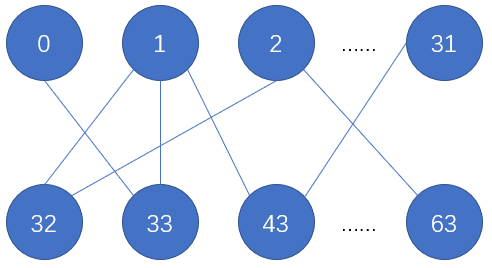
\includegraphics{figures/edge_generation}}%
	}
	\caption{Building Nodes.}
\end{figure}


\textbf{Edge Trimming}

There is a special edge in bipartite graph, which we call leaf edges. It can never be part of a cycle.
Leaf edges have a feature, the nodes it connects must have at least one node with the degree of the nodes being one.
By eliminating leaf edges in the bipartite graph, we can greatly reduce the complexity of the graph,
thus speeding up finding cycle from the bipartite graph.

\begin{figure}[ht]
	\centerline{%
		 \resizebox{0.8\textwidth}{!}{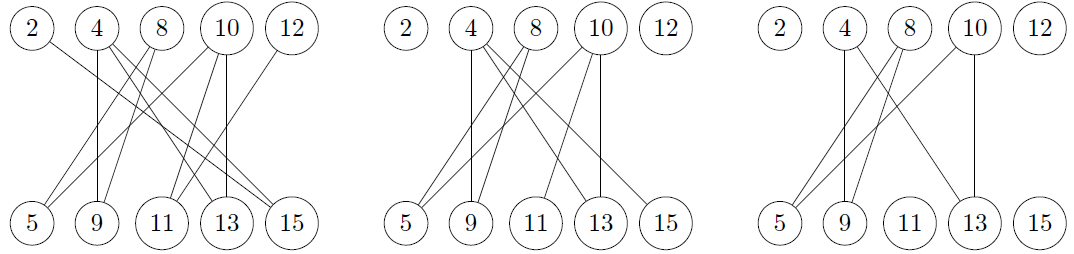
\includegraphics{figures/edge_trimming}}%
	}
	\caption{Trimming of edges which cannot be part of a cycle.}
\end{figure}

\begin{itemize}
	\item Step 1: node 0, node 3 and node 10 are one degree nodes, eliminating the edge (0,13), (6, 3) and the edge (10,9).
	\item Step 2: node 9 and node 13 are one degree nodes, eliminating the edge (8,9) and the edge (2,13).
	\item Step 3: node 8 is one degree nodes, eliminating the edge (8,11).
\end{itemize}


\textbf{Cycle detection}

After edge trimming, if a cycle of length L is found, we think we have found a solution to this problem.
we store the cycle edges in a set and put the nonce of the generated cycle in a set and
return as the result of cycle detection.


\textbf{Difficulty control}

The difficulty of finding a cycle in the graph is proportional to M/N. Here M stands for edges of the graph.
N stands for nodes of the graph. However, the difficulty of finding a cycle in the graph change is not smooth.
For crypto currencies, difficulty control must be scale in precisely controlled manner. The usual practice is
that the ratio of M/N remain fixed, such as M/N = 1/2.

Thus in the actual use, it also adds a hash difficulty control similar to Bitcoin. The digest of the cycle nonces is obtained by a hash function,
and then compared with the target difficulty.

\subsection{Rewards}
\subsubsection{Transaction Collision}
Due to asynchronous block submmission, BlockDAG protocols inevitably incorporate repeating transactions, called transaction collisons.
Miners tend to pack the transaction with higher fees to maximize their profit. This will result in high repetition rates of blocks. Repeated transactions will not contribute to the throughput, what is more, low fee transactions would wait indefinite time to get confirmed. In a fully decentralized network, nodes cannot coordinate each other to avoid collision, leaving the only option to deivse a sophiscated incentive mechanism to penalize the selfish mining behaviors.

The intuitive way to solve this problem is to share the transacation fee, and this method will make all the miners reach a Nash equilibrium that all the miners will choose transactions randomly from their memory pools. This approach will considerably reduce transactions collision; however, users can no longer pay higher fees to boost their transaction confirmation.

Qitmeer introduces an optimal incentive mechanism introduced in Inclusive\cite{Inclusive} protocol. It varies different transaction with different probability of being selected from memory pools, those with higher fee get higher probability. So, urgent transactions could increase their transaction fee to get better mining services, and low-fee transacations still get opportunity to confirm.

\subsubsection{First Come First Get}
To encourage miners to submit blocks immediately on creation. The transaction fee should belong to the first miner who incorporates it. So this reward machanism requires transactions has a global order, which has been offered by GHOSTDAG protocol.

Inclusive protocol states that this machanism has some security concerns because it won't penalize those malicious parites who mine blocks in private. Inclusive protocol fixes this problem by only giving rewards to blocks not deviating main chain too much. Qitmeer appreciates Inclusive protocol work and adopts it.

\section{Protocols and Interoperability}
BlockChain is the infrastructure for  decentralized finance. There will be an ecosystem when the blockchain becomes mature. This chapter introduces the typical applications on top of Qitmeer and the protocols for them to interact with Qitmeer.

\subsection{Mining Protocol}
\subsubsection{Proof-of-work Algorithm}

We hope to resist the centralization of mining power, and hope miner can utilizes almost all parts of commodity hardware (GPUs, CPUs).
Therefore, Qitmeer uses a Proof-Of-Work algorithm called Cuckoo Cycle\cite{cuckoocycle},
a memory-hard algorithm.This algorithm is designed to find certain subgraphs in large pseudo-random graphs.
An introduction of Qitmeer proof-of-work can be found here.\cite{qitmeerpow}

\subsubsection{Miner Capability}

At the moment, the fastest GPU miner implementation is Qitmeer-Miner, which developed by the Qitmeer developers.
However, the Qitmeer-Miner is still in the early stage of development, It's not a deeply optimized version. We hope
that the community will finally create more optimised miners.

The Qitmeer-Miner support parallel GPU. You can run multiple Nvidia GPUs and AMD GPUs mining in parallel.

Compatible GPU Hardware:

\begin{itemize}
\item Nvidia: GTX1060 GTX1070, GTX1070ti, GTX1080, GTX1080ti, GTX2070, GTX2080, GTX2080ti
\item AMD: RX570, RX580, Vega56, Vega64
\end{itemize}

In principle, as long as the graphics memory is greater than 5GB, the GPU miner can run.

The Qitmeer-Miner support both solo mining and pool mining.

\subsubsection*{Solo}
If you do decide to mine Qitmeer without joining a pool, these are the steps to achieve mining Qitmeer by yourself.

\begin{itemize}
\item You need to run a full node to validate transactions. First, install qitmeer\cite{qitmeer} with the complete blockchain downloaded. Qitmeer is a full node software program that fully validates transactions and blocks.
\item Download and install the Qitmeer miner software like Qitmeer-Miner. For a solo miner, the mining software connects to the blockchain full node (Qitmeer). The main job of the miner software is to create valid Proofs-of-Work and deliver the block to the rest of the Qitmeer network.
\item Finally, launch Qitmeer miner software and connect to Qitmeer network to start solo mining Qitmeer.
\end{itemize}

\subsubsection*{Pool}
Most mining pools support stratum protocol, so your miner program should be config this protocol.
For example:

\emph{miner.exe -o stratum+tcp://serverIp:3177 -m YourWalletAddress.YourMachineId}

\subsubsection{Mining Pool Capability}
The Proof-Of-Work algorithm implementation in Qitmeer is perfect for a mining pool.


\subsection{Wallet Protocol}
\subsubsection{Overview}
   The blockchain wallet itself does not store any digital currency, and is primarily a computer program for creating digital currency transactions, tracking balances, and making it easy for users to manage addresses and private keys. Wallet software is the foundation of the whole block chain ecological development, any industry service can be realized through a block chain wallet value, block chain technology itself will reconstruct the traditional Internet business model in its own way. After the release of Qitmeer on Testnet and Mainnet, the authorities will release the wallet application for different users at the same time. For example, in the professional-oriented command line wallet, users only need to input corresponding commands according to relevant instructions to complete address generation, send transactions and other operations; Mobile terminal wallet for ordinary users. Users can easily and quickly complete relevant operations on their mobile phones just like other apps.
\subsection*{Openness}
   An excellent blockchain public chain project should be more inclusive and open. Therefore, in addition to its own official wallet, Qitmeer has designed all interfaces and SDK for third-party wallet development at the beginning of development. Third party wallet institutions can use these interfaces to develop a variety of wallet programs that support Qitmeer Token transactions. Including: HD wallet, SPV wallet, browser wallet to meet a variety of user needs.
\subsection*{How to create a wallet}
   The following is a simple wallet creation and transaction steps:
\begin{enumerate}
	\item  Generate seeder.
    \item  Derive private key.
    \item  Derive public key.
    \item  Derive address.
    \item  Monitor for outputs.
    \item  Create unsigned Txes.
    \item  Sign Txes.
    \item  Broadcast Txes.
\end{enumerate}

   To complete the above operations, we need to rely on qitmeer's nx SDK and RPC interface.
   The NX SDK is a collection of tools that integrates various encryption, decryption, and signature functions. We can use the nx SDK to develop the following functions:
   \begin{enumerate}
     \item Generate seeder.
     \item Derive private key.
     \item Derive public key.
     \item Derive address.
     \item Create unsigned Txes.
	 \item Sign Txes.
   \end{enumerate}

   RPC is an http-based network interface, it’s easy to interaction with qitmeer network. We can use the nx SDK to develop the following functions:

   \begin{enumerate}
    \item  Get block count from block dag or block chain.
    \item Get block data with block height.
    \item  Gettransaction data with txid.
    \item  Gets all transaction data waiting for confirmation.
    \item  Monitor for outputs.
    \item  Broadcast Txes.
   \end{enumerate}


\subsection{Cross Chain}
Qitmeer is dedicated tp undertake the liquidity of whole Ismalic decentralized finance. So the design goal of Qitmeer is to build a simple and strong UTXO-based value transfer network, that is why Qitmeer itself doesn't provide an on chain smart contract for the simplicity; instead, it prefers interoperability solutions to integrate various blockchains and applications. Finally, they will be parts of Qitmeer's ecosystem and can interact with each other.

\subsubsection{UTXO interoperability}

Across the chain technology is mainly to solve different main chain (such as: ` HLC ` and ` BTC `) problem of data exchange between the most direct cross chain technology application is "DEX :distributed exchange", No third party participation will purse ` BTC ` into ` HLC `,Complete wallet-to-wallet transactions.

Currently, Qitmeer has supported P2SH script contracts and cross-chain functions through hash-locking.

\subsubsection*{Principle}

The implementation process of hash locking across the chain is:

\begin{enumerate}
\item  Alice and Bob generate their respective addresses on 'HLC' and 'BTC' chains respectively;

\item Alice generates her own Secret Key and Secret Key hash;

\item Alice locks her 'HLC' token into the hash lock contract in the main chain of 'HLC'. The unlock condition is that Bob holds the Secret Key or returns it to Alice after exceeding the specified time;

\item Bob checks the contract of Alice's main chain in 'HLC' and USES to generate the corresponding contract in 'BTC'. The unlock condition is that Alice holds the Secret Key or returns it to Bob after the specified time;

\item Alice USES to remove Bob's lock 'BTC' in the hash lock contract;

\item After obtaining , Bob locks Alice 'HLC' in the hash lock contract, and completes the transaction;

\end{enumerate}

\begin{figure}[hbt]
	\centerline{%
	   \resizebox{0.8\textwidth}{!}{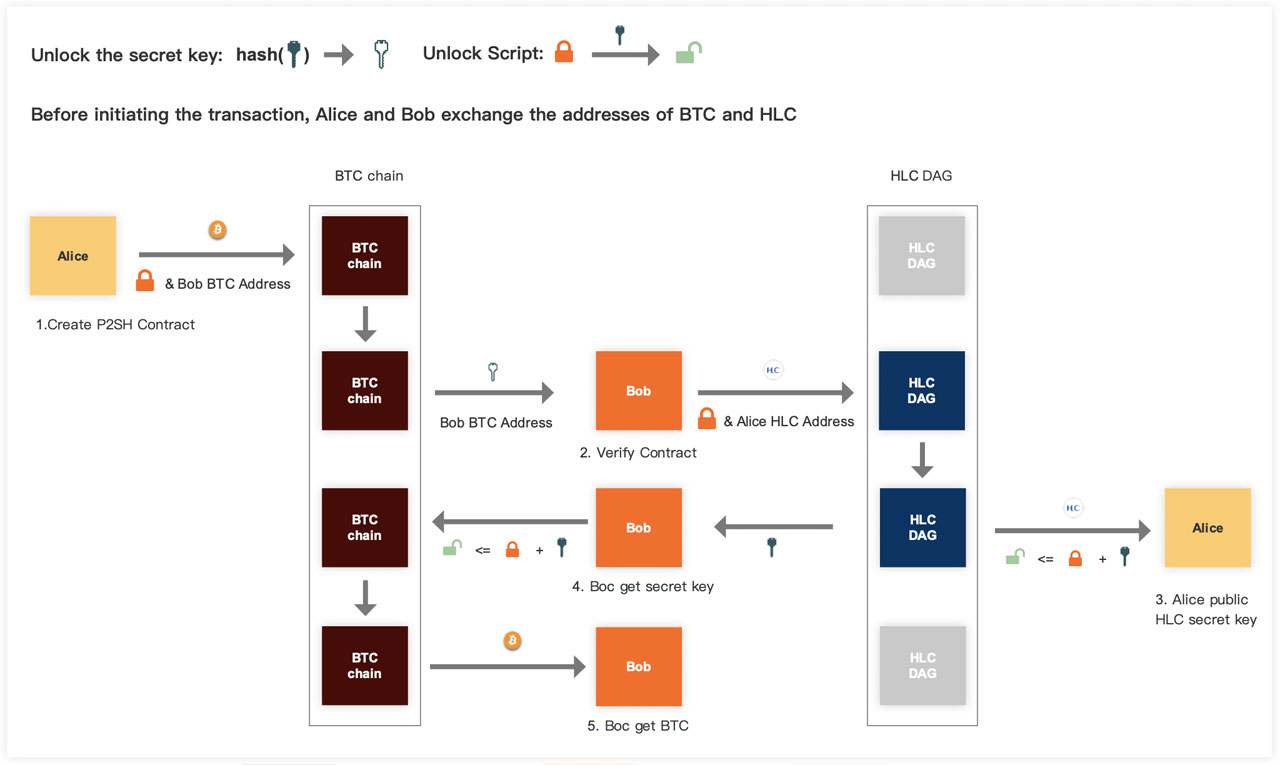
\includegraphics{figures/UTXOAtomicSwap.jpg}}%
	}
\caption{UTXO}
\end{figure}



\subsubsection{Smartcontract interoperability}

Based on the cross-chain solution of intelligent contract type, Qitmeer completes the cross-chain transaction of the block chain assets of Qitmeer to other account models through hash lock Smartcontract.

The following will take EHT as an example to illustrate how to complete the cross-chain operation of Smartcontract.

\subsubsection*{Smartcontract interoperability Principle}

\begin{enumerate}
\item  Alice and Bob generate their respective addresses on 'HLC' and 'ETH' chains respectively;

\item   Alice generates her own Secret Key and Secret Key hash;

 \item  Alice locks her 'HLC' token into the hash lock contract in the main chain of 'HLC'. The unlock condition is that Bob holds the Secret Key or returns it to Alice after exceeding the specified time;

 \item  Bob checks the contract of Alice in the main chain of 'HLC' and generates the corresponding contract on 'ETH' using a . The unlock condition is that Alice holds the Secret Key or returns it to Bob after exceeding the specified time.

 \item  Alice USES to call Smartcontract to remove 'ETH';

 \item  After obtaining , Bob locks Alice 'HLC' in the hash lock contract, and completes the transaction;

\end{enumerate}


\clearpage
%\appendix
%\section{Appendix}
%\begin{appendices}
%\section{append A}

%Foo bar Foo bar Foo bar Foo bar Foo bar Foo bar Foo bar Foo bar Foo bar Foo bar

%\end{appendices}

%\bibliographystyle{plainnat}
%\bibliographystyle{unsrt,acm}
\bibliographystyle{unsrt}
\bibliography{hlc_whitepaper}

\end{document}

